%!TEX root = skripsi.tex
%-----------------------------------------------------------------------------%
\chapter{\babTiga}
%-----------------------------------------------------------------------------%
Bab ini akan menjelaskan gambaran proses penelitian secara keseluruhan yang sesuai dengan rancangan sistem pada gambar \ref{fig:Rancangan-Sistem}.

\begin{figure}
	\centering
	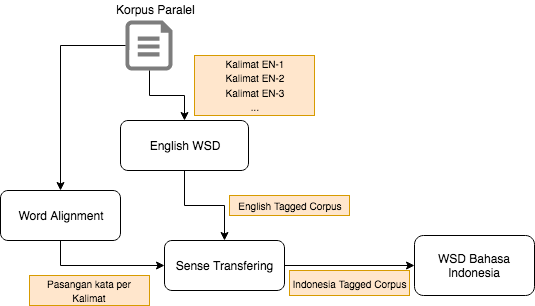
\includegraphics[width=1\linewidth]{adit_pics/WSD-full}
	\caption{Rancangan Sistem}
	\label{fig:Rancangan-Sistem}
\end{figure}

Proses \textit{pipeline} terdiri dari pembuatan \textit{sense tagged corpus} bahasa Inggris,  \textit{word alignment} korpus paralel, peningkatan kualitas dan evaluasi \textit{word alignment}, pemindahan \textit{sense} dari korpus bahasa Inggris, dan sistem WSD yang diimplementasikan.
%-----------------------------------------------------------------------------%

\section{Pembuatan \textit{Sense Tagged Corpus} Bahasa Inggris}
%-----------------------------------------------------------------------------%

Pembuatan \textit{sense tagged corpus} bahasa Inggris dilakukan dengan menggunakan \textit{tool} IMS \citep{zhong2010makes} untuk mendapatkan makna terbaik yang dapat ditag oleh \textit{tool} tersebut. Makna kata hasil dari proses ini akan dipindahkan ke kata yang bersesuaian pada kalimat yang sama pada bagian \textit{sense transfering}. \textit{File} yang diberikan sebagai masukan dari IMS adalah kalimat-kalimat pada bahasa Inggris yang berasal dari korpus identik.
%-----------------------------------------------------------------------------%
\section{\textit{Word alignment} pada Korpus Paralel}
%-----------------------------------------------------------------------------%
Proses \textit{word alignment} ini dilakukan agar nantinya makna kata dari suatu kata dalam bahasa Inggris dapat ditransfer ke kata yang bersesuaian pada Bahasa Indonesia.

Proses \textit{alignment} yang dilakukan dengan Giza++ meliputi tahap-tahap berikut:
\begin{enumerate}
	\item Mempersiapkan kedua buah \textit{file} yaitu korpus bahasa asal (\textit{source}) dan korpus bahasa tujuan (\textit{target}). Kedua \textit{file} ini berpasangan dalam setiap barisnya. Baris pertama dalam \textit{file} pertama berpasangan dengan baris pertama pada \textit{file} kedua sampai akhir baris pada kedua \textit{file}.
	\item Menghasilkan \textit{file} perbendaharaan kata dari kedua bahasa dan \textit{list} indeks perbendaharaan kata pada tiap kalimat yang sudah diselaraskan
	\item Menghasilkan \textit{cooccurence file} dari kosa kata dan pasangan kalimat tersebut
	\item Proses \textit{alignment} yang menghasilkan beberapa macam \textit{output file} 
\end{enumerate}

Terdapat satu buah \textit{output file} Giza++ yang berisi pasangan-pasangan kalimat dengan kata-kata yang sudah diselaraskan dengan translasinya dalam bahasa tujuan. Hasil ini merupakan \textit{best viterbi alignment} menurut Giza++.

Pada skenario \textit{alignment} dengan bahasa Indonesia sebagai \textit{source} dan bahasa Inggris sebagai \textit{target}, satu kata dalam bahasa Indonesia akan dipasangkan dengan tepat satu kata dalam bahasa Inggris.

%-----------------------------------------------------------------------------%

\section{Peningkatan Kualitas Hasil \textit{Alignment}}
%-----------------------------------------------------------------------------%
Proses peningkatan kualitas hasil alignment diperlukan untuk meminimalisir kesalahan pemasangan kata-kata pada proses sebelumnya. Permasalahan  yang terjadi adalah adanya pasangan-pasangan kata yang tidak benar seperti pada halnya kata "lapangan" misalnya yang  dipasangkan dengan kata dalam bahasa inggris \textit{field}, \textit{ground}, \textit{involved}, \textit{job}, \textit{program}, dan beberapa kata lainnya. Peningkatan kualitas \textit{alignment} ini dilakukan dengan dua buah pendekatan, yaitu dengan bantuan \textit{online dictionary} bahasa Indonesia-Inggris dan \textit{bi-directional alignment}. 

Pendekatan dengan bantuan kamus diterapkan dengan mencari kata terjemahan pada bahasa Inggris untuk menentukan apakah \textit{alignment} benar atau salah. Pada pendekatan kedua, dilakukan \textit{inverse} \textit{alignment} antara bahasa Indonesia ke Inggris. Jika pada proses awal \textit{alignment} dilakukan dengan menerapkan bahasa Indonesia sebagai \textit{source} dan Inggris sebagai \textit{target}, kali ini dilakukan proses yang berkebalikan. Pemanfaatkan hasil \textit{alignment} korpus bahasa Inggris ke Indonesia akan menghasilkan pasangan-pasangan kata dengan tingkat kesalahan \textit{alignment} lebih kecil dari \textit{alignment} satu arah saja. Metode yang akan dilakukan adalah dengan memeriksa setiap pasangan kata dari bahasa Indonesia yang mana merupakan kata dalam bahasa Inggris, apakah kata tersebut memiliki pasangan dalam \textit{inverse alignment} Giza.

%-----------------------------------------------------------------------------%
\section{\textit{Sense Transfering}} \label{sec:Sense Transfering}
%-----------------------------------------------------------------------------%
Pemindahan makna kata dilakukan dengan beberapa \textit{sub-process} yang terdiri dari pemasangan antar kalimat, pemeriksaan kata, dan \textit{sense transfering}.
\begin{enumerate}
	\item Pemasangan antar kalimat yang bersesuaian dengan kata-kata yang berpasangan. Pada contoh kata "halaman" yang berpasangan dengan "courtyard", maka pasangan kalimat "Aku bermain di halaman" akan dipasangkan dengan kalimat "I play at the courtyard". Pemeriksaan untuk kata yang saling berpasangan menggunakan hasil dari \textit{alignment} dan kamus hasil \textit{alignment enhancement}.
	\item \textit{Sense} dari kata yang menjadi \textit{target} tersebut ("halaman") kemudian diperiksa dengan \textit{sense} kata yang sama yang sudah pernah dipindahkan dari pasangan kalimat lain. Jika \textit{sense} yang ingin dipindahkan "mirip" dan memiliki kedekatan makna diatas batas \textit{threshold}, maka \textit{sense} yang akan dipindahkan hanya salah satunya saja. Proses ini diperlukan untuk meminimalisir adanya satu kata bahasa Indonesia yang mempunyai lebih dari satu \textit{sense} yang mirip dari definisi makna tersebut.
	\item Pemindahan makna dilakukan sebagai proses akhir. Bila "courtyard" memiliki \textit{sense} yang artinya adalah "pekarangan rumah", maka "halaman" pada kalimat "Aku bermain di halaman" memiliki \textit{sense} "pekarangan rumah".
\end{enumerate}

\section{Sistem WSD} \label{sec:Sistem WSD}
%-----------------------------------------------------------------------------%
Sistem WSD yang dibangun adalah dengan menggunakan pendekatan \textit{supervised learning}. \textit{Classifier} yang digunakan dalam sistem \textit{WSD} ini adalah SVM dengan fitur-fitur tertentu. Pengujian dilakukan dengan menggunakan beberapa fitur seperti \textit{bag of words}, \textit{POS Tag}, dan \textit{word embedding}. Fitur \textit{bag of words} menggunakan \textit{window} sebanyak dua buah kata kanan dan kiri kata tujuan sebagai kata konteks. Fitur \textit{POS Tag} dan vektor \textit{word embedding} juga akan dicoba sebagai skenario pada penelitian ini.

\section{Evaluasi}

Terdapat evaluasi khusus untuk proses \textit{word alignment} dan sistem WSD Bahasa Indonesia yang dibangun. Evaluasi pada bagian \textit{word alignment} ditujukan untuk mengetahui seberapa baik dan \textit{reliable} proses \textit{alignment} yang dilakukan Giza++. Sementara itu, sistem WSD dievaluasi untuk mendapatkan gambaran performa dari fitur seperti apa yang memberikan akurasi terbaik.

\subsection{\textit{Word Alignment}}
\textit{Word alignment} hasil dari \textit{tool} Giza++ dievaluasi dengan membandingkan hasil \textit{alignment} dari \textit{anotator}(orang yang melakukan evaluasi \textit{alignment} secara manual) dengan hasil \textit{alignment} Giza. Hasil \textit{alignment} yang dilakukan anotator akan dijadikan sebagai \textit{gold standard} acuan untuk perbandingan. Nilai-nilai yang akan dihitung meliputi \textit{precision} (P), \textit{recall} (R), dan F-\textit{score}. 

\subsubsection{Proses Anotasi}

Anotator diberikan panduan untuk melakukan anotasi sesuai dengan \textit{task} yang dilakukan Giza. Kedua anotator diminta untuk memasangkan kata-kata yang bersesuaian untuk masing-masing kalimat (dalam bahasa Inggris dan Indonesia) dengan format \textit{file} yang mirip dengan Giza. Panduan anotasi yang diberikan dapat dilihat pada lampiran.

\subsubsection{Proses Evaluasi}

Hasil \textit{alignment} dari kedua anotator masing-masing dibandingkan dengan hasil \textit{alignment} yang dilakukan oleh Giza. Perhitungan Precision, Recall, dan F-score dihitung berdasarkan perbandingan seberapa banyak \textit{alignment} yang benar dengan banyaknya \textit{alignment} yang dilakukan. Proses lebih rinci dari perhitungan yang dilakukan akan dijelaskan pada Bab 4.

\subsection{Sistem WSD}
Hasil dari \textit{sense transfering} akan digunakan sebagai \textit{training} dan \textit{testing} data untuk menguji performa dari sistem yang dibangun. Performa dari sistem WSD akan dilihat berdasarkan perhitungan F1-score dari hasil klasifikasi makna kata yang dilakukan dengan menggunakan \textit{cross validation}.